\section{Paging}

\paragraph{Hierarchical Page Table --- two-level page table}
\begin{items}
  \item \textbf{layout}: on 32-bit machine with 4KiB pages divide virtual address into \\*
    $ - $ \emph{page number} (p): 20 bits \\*
    $ - $ \emph{page offset} (d): 12 bits
  \item \textbf{table paging}: table can be paged to save memory -- subdivide vpn: \\*
    $ - $ index in \emph{page directory} ($ p_1 $): 10 bits \\*
    $ - $ index in \emph{page table entry} ($ p_2 $): 10 bits
  \item for ranges of 1024 invalid pages, reset present bit in page directory \\*
    $ \to $ save space of second-level page table
\end{items}
\begin{figure}[H]\centering\label{TwoLevelPageTable}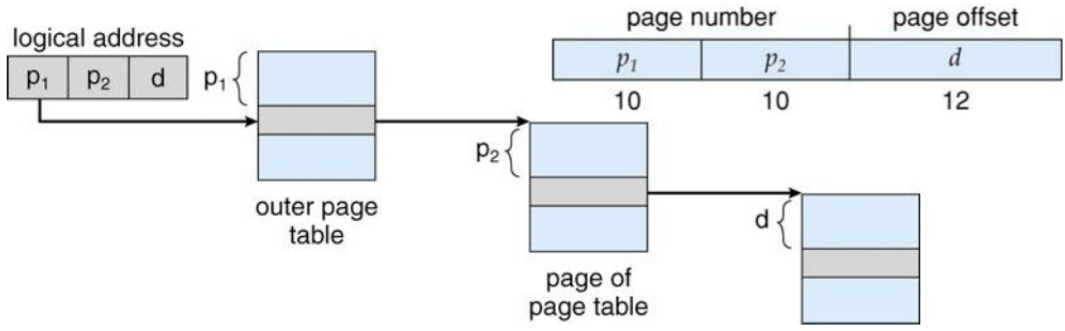
\includegraphics[width=0.33\textwidth]{TwoLevelPageTable}\end{figure}

\paragraph{Linear Inverted Page Table}
\begin{items}
  \item \textbf{Problem}: large AS (64 bit) but only few mapped virtual addresses \\*
    $ \to $ much memory wasted on page tables \\*
    $ \to $ lookup slow due to many levels of hierarchy
  \item \textbf{Idea}: invert page table mapping \\*
    $ - $ map physical frame to virtual page instead of other way around \\*
    $ - $ single page table for \emph{all processes} (exactly one table per system) \\*
    $ - $ one page table entry for each physical page frame
  \item \textbf{Advantage}: less overhead for page table meta data
  \item \textbf{Disadvantage}: increases time needed to search table when page reference occurs
\end{items}
\begin{figure}[H]\centering\label{LinearInvertedPageTable}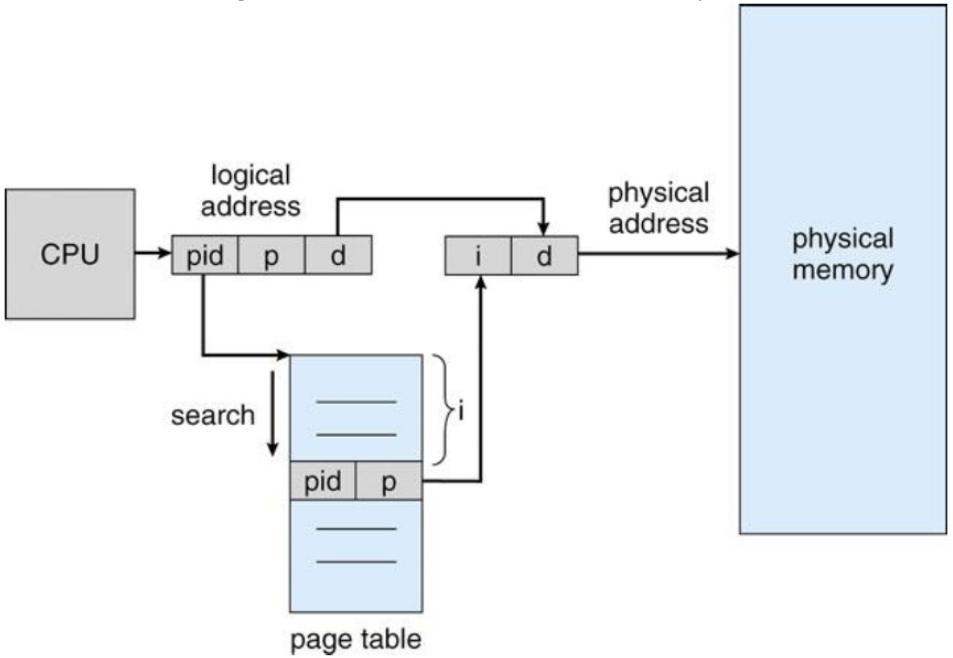
\includegraphics[width=0.33\textwidth]{LinearInvertedPageTable}\end{figure}

\paragraph{Hashed Inverted Page Table}
\begin{items}
  \item \textbf{hash anchor table}: limits search to at most a few page-table entries
\end{items}

\paragraph{Translation Lookaside Buffer --- motivation}
\begin{items}
  \item \textbf{naive paging is slow}: \\*
    $ - $ every load/store requires multiple memory references \\*
    $ - $ 4-level hierarchy: 5 memory references for every load/store \\* \phantom{$ - $} \phantom{$ \cdot $} (4 page directory/table references, 1 data access)
  \item \textbf{Idea}: add cache that stores recent memory translations \\*
    $ - $ \emph{translation lookaside buffer} (TLB) maps [vpn] to [pfn, protection] \\*
    $ - $ typically 4-way to fully associative hardware cache in MMU \\*
    $ - $ typically 64-2000 entries \\*
    $ - $ typically 95\%-99\% hit rate
\end{items}

\paragraph{TLB --- operation}
\begin{items}
  \item on every load/store: \\*
    $ - $ check if translation result is cached in TLB (\emph{TLB hit}) \\*
    $ - $ otherwise walk page tables, insert result into TLB (\emph{TLB miss})
  \item \textbf{Quick}: can compare many TLB entries in parallel in hardware
\end{items}

\paragraph{TLB --- TLB miss}
\begin{items}
  \item \textbf{Process}: \\*
    $ - $ evict entry from TLB on TLB miss \\*
    $ - $ load entry for missing virtual address into TLB
  \item \textbf{Variants}: \emph{software-managed} and \emph{hardware managed}
  \item \textbf{software-managed TLB}: \\*
    $ - $ OS receives \emph{TLB miss exception} \\*
    $ - $ OS decides which entry to evict (drop) from TLB \\*
    $ - $ OS generally walks page tables in software to fill new TLB entry \\*
    $ - $ TLB entry format specified in \emph{instruction set architecture} (ISA)
  \item \textbf{hardware-managed TLB}: \\*
    $ - $ evict TLB entry based on hardware-encoded policy \\*
    $ - $ walk page table in hardware $ \to $ resolve address mapping
\end{items}

\paragraph{TLB --- address space identifiers}
\begin{items}
  \item \textbf{Problem}: vpn dependent on AS \\*
    $ - $ vpns in different AS can map to different pfns \\*
    $ \to $ need to clear TLB on AS switch
  \item \textbf{Idea}: solve vpn ambiguity with additional identifiers in TLB
  \item \textbf{ASID}: TLB has \emph{address space identifier} (ASID) in every entry \\*
    $ - $ map [vpn, ASID] to [pfn, protection] \\*
    $ \to $ avoids TLB flush at every address-space switch \\*
    $ \to $ less TLB misses: some TLB entries still present from last time process ran
\end{items}

\paragraph{TLB --- reach}
\begin{items}
  \item = amount of memory accessible with TLB hits: \\*
    $ \text{TLB reach} = \text{TLB size} * \text{page size} $
  \item \textbf{ideally}: working set of each process is stored in TLB (otherwise high degree of TLB misses)
  \item \textbf{increase page size}: \\*
    $ + $ fewer TLB entries per memory needed \\*
    $ - $ increase internal fragmentation
  \item \textbf{multiple page sizes}: \\*
    $ + $ allows applications that map larger memory areas to increase TLB coverage with minimal \\* \phantom{$ + $} fragmentation increase
  \item \textbf{increase TLB size}: \\*
    $ - $ expensive
\end{items}

\paragraph{TLB --- effective access time}
\begin{items}
  \item \textbf{associative lookup}: takes $ \tau $ time units (e.g., $ \tau = 1\text{ns} $)
  \item \textbf{memory cycle}: takes $ \mu $ time units (e.g., $ \mu = 100\text{ns} $)
  \item \textbf{TLB hit ratio} $ \alpha $: percentage of all memory accesses with cached translation (e.g., $ \alpha = 99\% $)
  \item \textbf{effective access time} (EAT) for linear page table without cache: \\*
    $ \text{EAT} = (\tau + \mu)\alpha + (\tau + 2\mu)(1-\alpha) = \tau + 2\mu - \mu\alpha $
\end{items}

\begin{summary}
  \begin{items}
    \item page tables communicate between OS and MMU hardware  \\*
      $ - $ how virtual addresses in each address space translate to physical addresses \\*
      $ - $ which kind of accesses the MMU should allow/signal to the OS
    \item different page table layouts have been developed  \\*
      $ - $ linear page table \\*
      $ - $ hierarchical page tables \\*
      $ - $ inverted page tables \\*
      $ - $ hashed page tables
    \item performing page table lookups for every memory access significantly slows down execution time of programs \\*
    $ - $ translation lookaside buffer (TLB) caches previously performed page table lookups \\*
    $ - $ typical TLBs cover $ 95\%-99\% $ of all translations
  \end{items}
\end{summary}